\documentclass{webofc}
\usepackage[varg]{txfonts}
\usepackage{xspace}
\usepackage{hyperref}

\newcommand{\tauo}{\ensuremath{c\tau_{0}}\xspace}
\newcommand{\ctau}{\ensuremath{c\tau_{0}}\xspace}
\newcommand{\gluino}{\ensuremath{\tilde{\textrm{g}}}\xspace}
\newcommand{\lsp}{\ensuremath{\tilde{\chi}_{1}^{0}}\xspace}

\begin{document}

\title{Identification of new long-lived particles using a deep neural network}

\author{\firstname{Matthias} \lastname{Komm} \inst{1}\fnsep\thanks{\email{Matthias.Komm@cern.ch}}, for the CMS Collaboration}

\institute{Imperial College London, Physics Department, SW7 2BW London, United Kingdom}

\abstract{
We present the development of a deep neural network for identifying generic displaced jets arising from the decays of new long-lived particles in data recorded by the CMS detector at the CERN LHC. Various jet features including detailed information about each clustered candidate as well as reconstructed secondary vertices are refined through the use of 1-dimensional convolution layers before being combined with high-level engineered features and passed through a series of fully-connected layers. The lifetime, \tauo, is treated as a parameter of the neural network model, which allows for hypothesis testing over several orders of magnitude ranging from $\ctau = 1\,\mu\textrm{m}$ to 10\,m. Domain adaptation by backward propagation is performed to construct domain-independent features at an intermediate layer of the network to mitiage difference between simulation and data. The training is performed by streaming ROOT trees containing $\mathcal{O}$(100M) jets directly into the TensorFlow queue and threading system allows a flexible selection of input features and the asynchronous preprocessing of data, such as the resampling and shuffling of batches on the CPU, in parallel to training on the GPU. The performance of the tagger is demonstrated in a search for long-lived gluinos as predicted by split supersymmetric models.
}

\maketitle
%
\section{Introduction}
\label{intro}

Machine-learned algorithms are routinely deployed to perform event reconstruction, particle identification, event classification, and other tasks~\cite{ml-white-paper} when analysing data samples recorded by experiments at the CERN LHC. For example, the ATLAS~\cite{atlas} and CMS~\cite{cms} Collaborations have developed numerous algorithms based on boosted decision trees or neural networks to identify jets originating from the hadronisation of bottom quarks with unprecedented performance~\cite{batlas,bcms}.

This note, based on Ref.~\cite{CMS-EXO-19-011}, summarises the development and application of a novel algorithm for identifying jets originating from the decay of long-lived particles (LLPs). The algorithm is based on a deep neural network (DNN) that is inspired by the CMS DeepJet approach~\cite{dj}, albeit several aspects required an extension of the DeepJet architecture and training procedure. To perform supervised learning a generic definition for displaced jets is introduced. Furthermore, the DNN is parametrised as a function of the proper lifetime, \tauo, of the long-lived particle to allow hypothesis testing over several orders of magnitude ranging from $\ctau = 1\,\mu\textrm{m}$ to 10\,m. To mitigate uncertainties arising from difference between simulation and data, domain adaptation by backward propagation~\cite{da} is applied during the training. The application of the resulting DNN is demonstrated in a search for long-lived gluino production as predicted by split supersymmetric (SUSY) models~\cite{splitsusy}.

\section{Simulated samples and jet labelling}
\label{samples}

Jets from the hadronisation of gluon, light quarks (uds), charm, and bottom quarks are used as background classes in the DNN training. These are taken from simulated samples of multijet events produced via the strong interaction, a manifestation of quantum chromodynamics (QCD), and of top quark pair production. Signal jets from LLP decays are taken from various samples of simulated events containing pair-produced long-lived gluinos (\gluino) that decay into a light quark/antiquark pair and a neutralino (\lsp) with varying lifetime and gluino and neutralino masses. At the LLP decay vertex, the two quarks can still interact which each other leading often to more than only two distinct jets as shown for two example decays in Fig.~\ref{decay}.

\begin{figure*}[!ht]
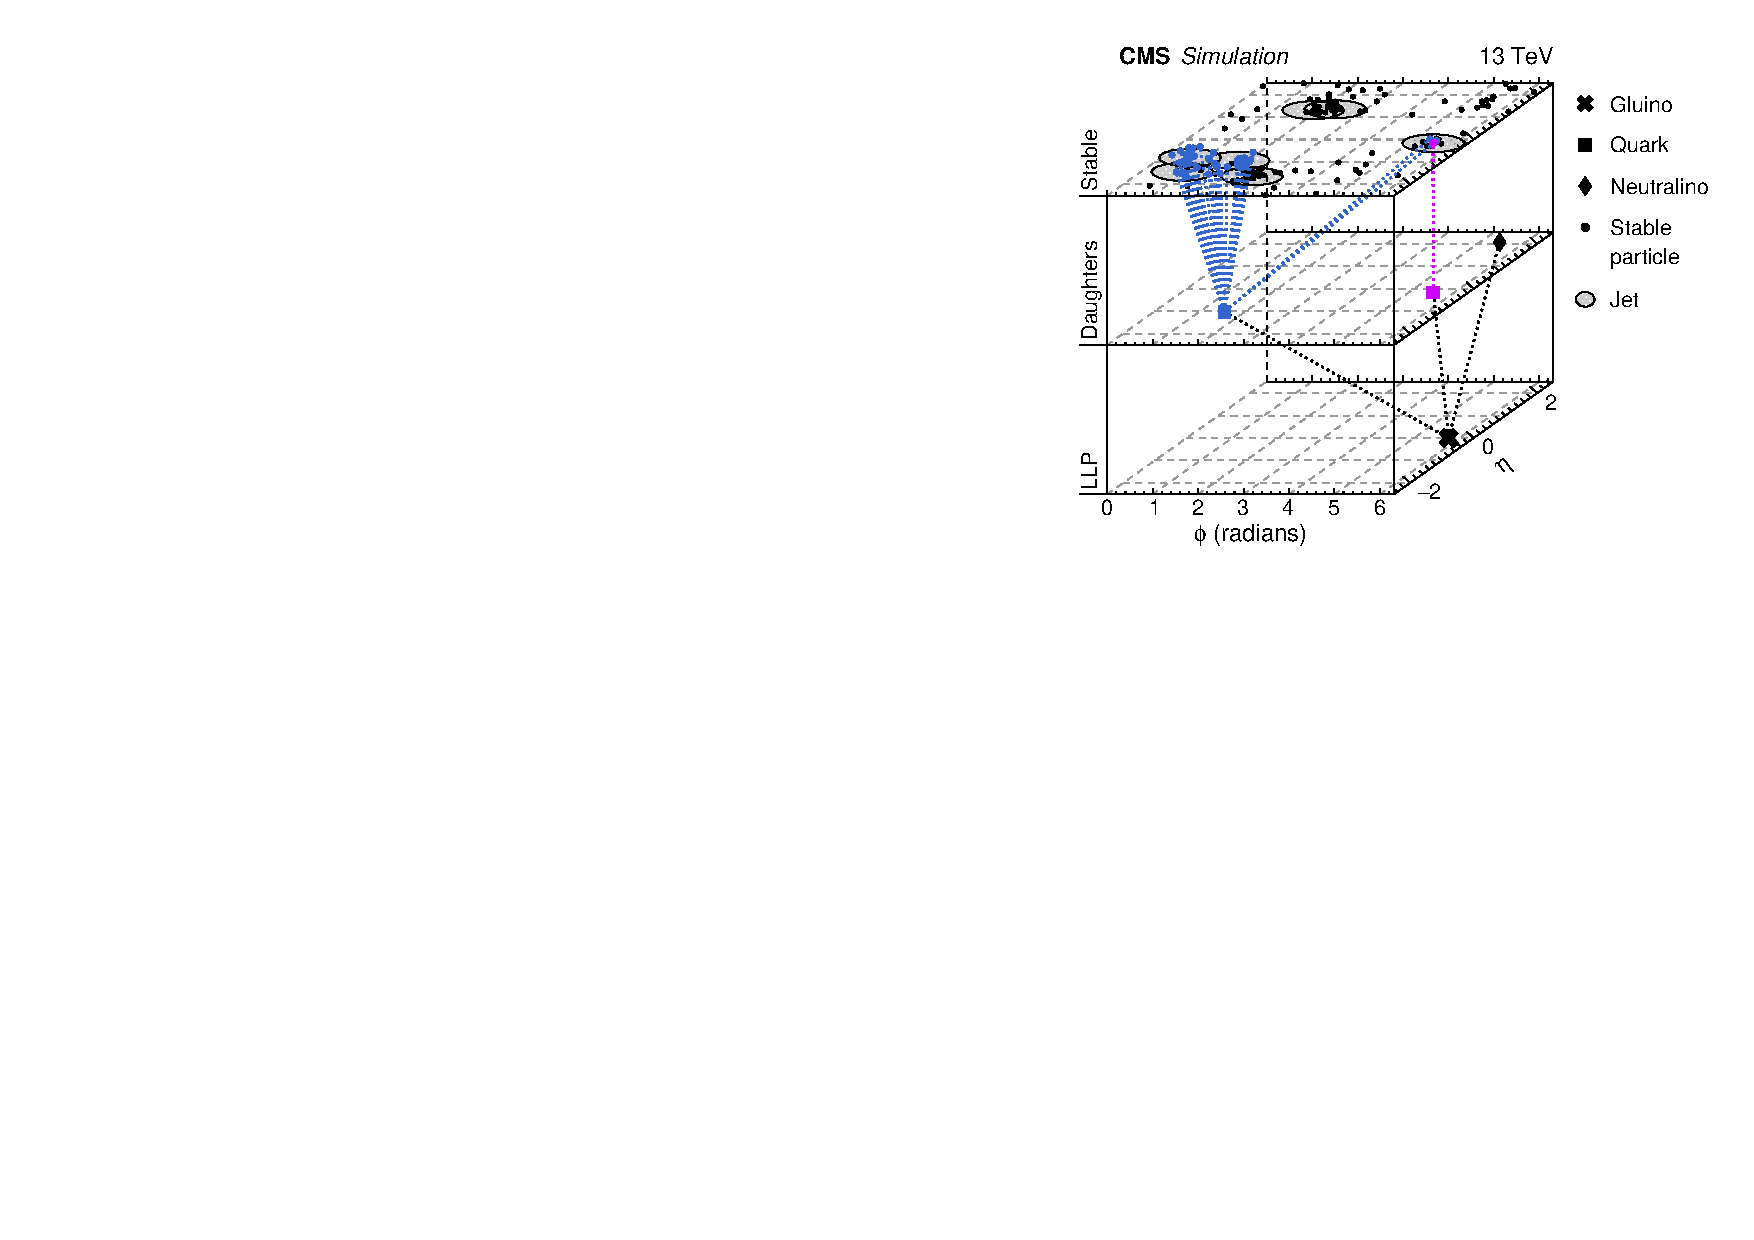
\includegraphics[width=0.48\textwidth]{figs/decay1.pdf}\hspace{0.03\textwidth}
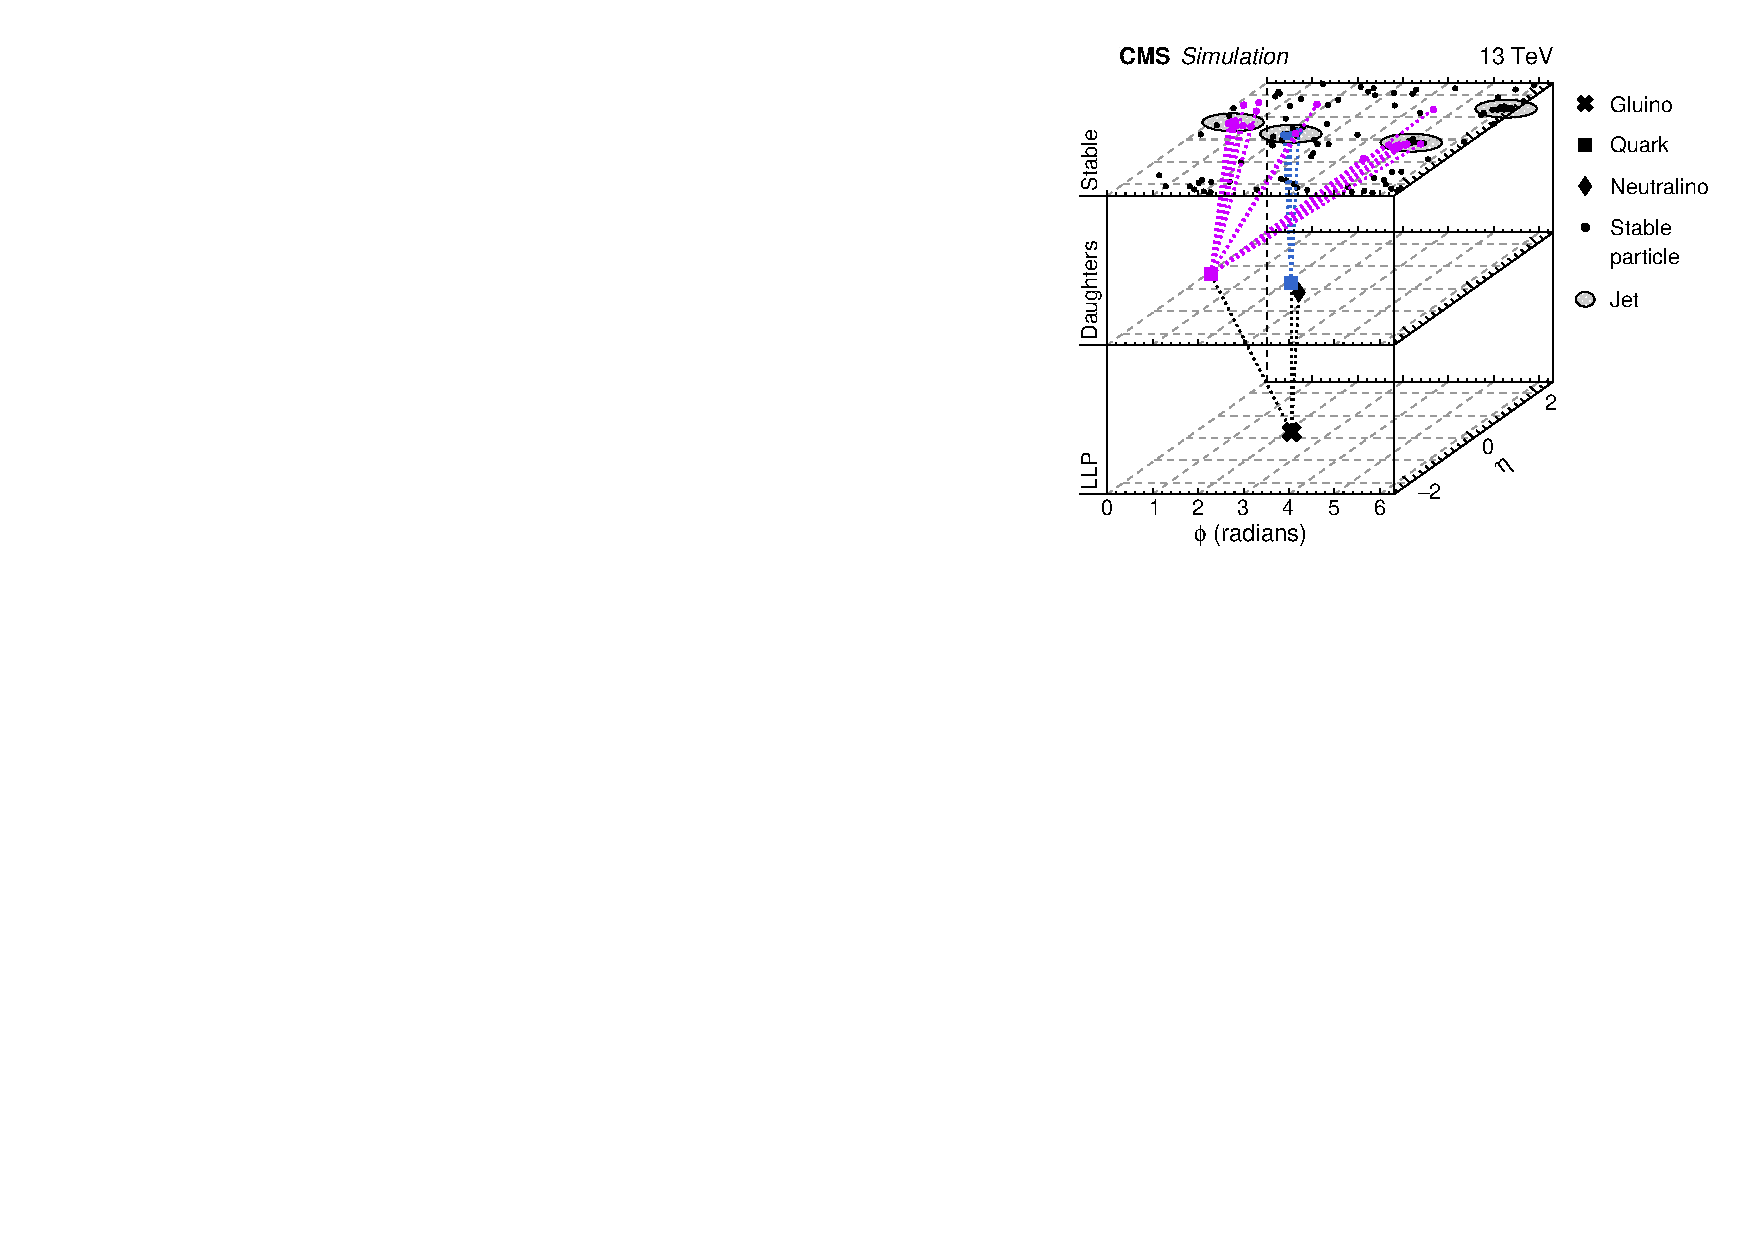
\includegraphics[width=0.48\textwidth]{figs/decay2.pdf}
\centering
\caption{Two example gluino decays into a quark/antiquark pair and a neutralino. The positions in $\eta$ and $\phi$ of the gluino, the quarks and neutralino, and the jets clustered from the stable particles after hadronisation are shown in the lower, middle and top layer, respectively. The figures are taken from Ref.~\cite{CMS-EXO-19-011}.}
\label{decay}
\end{figure*}

A novel definition of a generic LLP jet is introduced by labelling only those jets as 'LLP' for which most of the momentum is carried by clustered particles stemming from the gluino decay vertex, determined from generator-truth information.


\section{Deep neural network architecture and training}
\label{dnn}

An overview of the DNN architecture is given in Fig.~\ref{arch}. Approximately 600 input features are considered. The features of the clustered charged and neutral jet constituents and secondary vertices are compressed through a series of one-dimensional convolutions with a kernel size of one. After flattening, these are combined with the LLP lifetime and global jet features. After a single dense layer with 200 nodes the network is split in two parts. The top part attempts to predict the jet label whereas the bottom part predicts the domain of a jet, i.e. if a jet stems from data or simulation. Domain adaptation by backward propagation~\cite{da} is performed by reversing the gradients of the domain loss with respect to the network weights in the preceding layers as indicated. When minimising the combined loss $L_\mathrm{class}+L_\mathrm{domain}$, the network is forced to only retain features that are domain-invariant. The strength of this effect is be controlled through the hyperparameter $\lambda$.

\begin{figure*}[!ht]
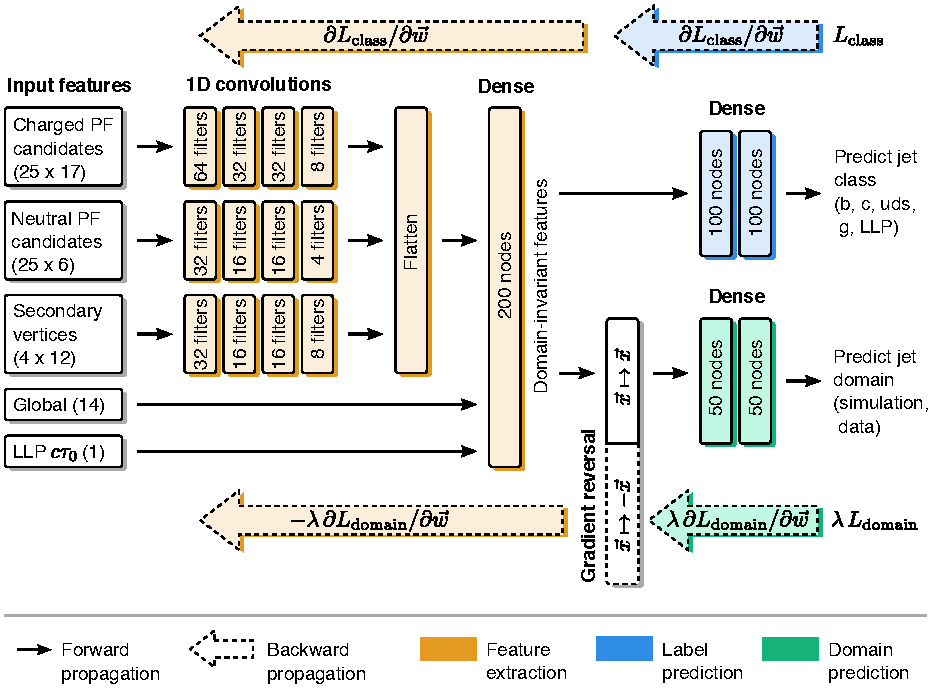
\includegraphics[width=0.9\textwidth]{figs/network.pdf}
\centering
\caption{An overview of the DNN architecture, which comprises convolutional and dense layers; the numbers of filters and nodes are indicated. The input features are grouped by object type and ($m\times n$) indicates the maximum number of objects ($m$) and the number of features per object ($n$). The gradients of the class ($L_\textrm{class}$) and domain ($L_\textrm{domain}$) losses with respect to the weights $w$, used during backward propagation, are shown. The figure is taken from Ref.~\cite{CMS-EXO-19-011}.}
\label{arch}
\end{figure*}

\begin{figure*}[!ht]
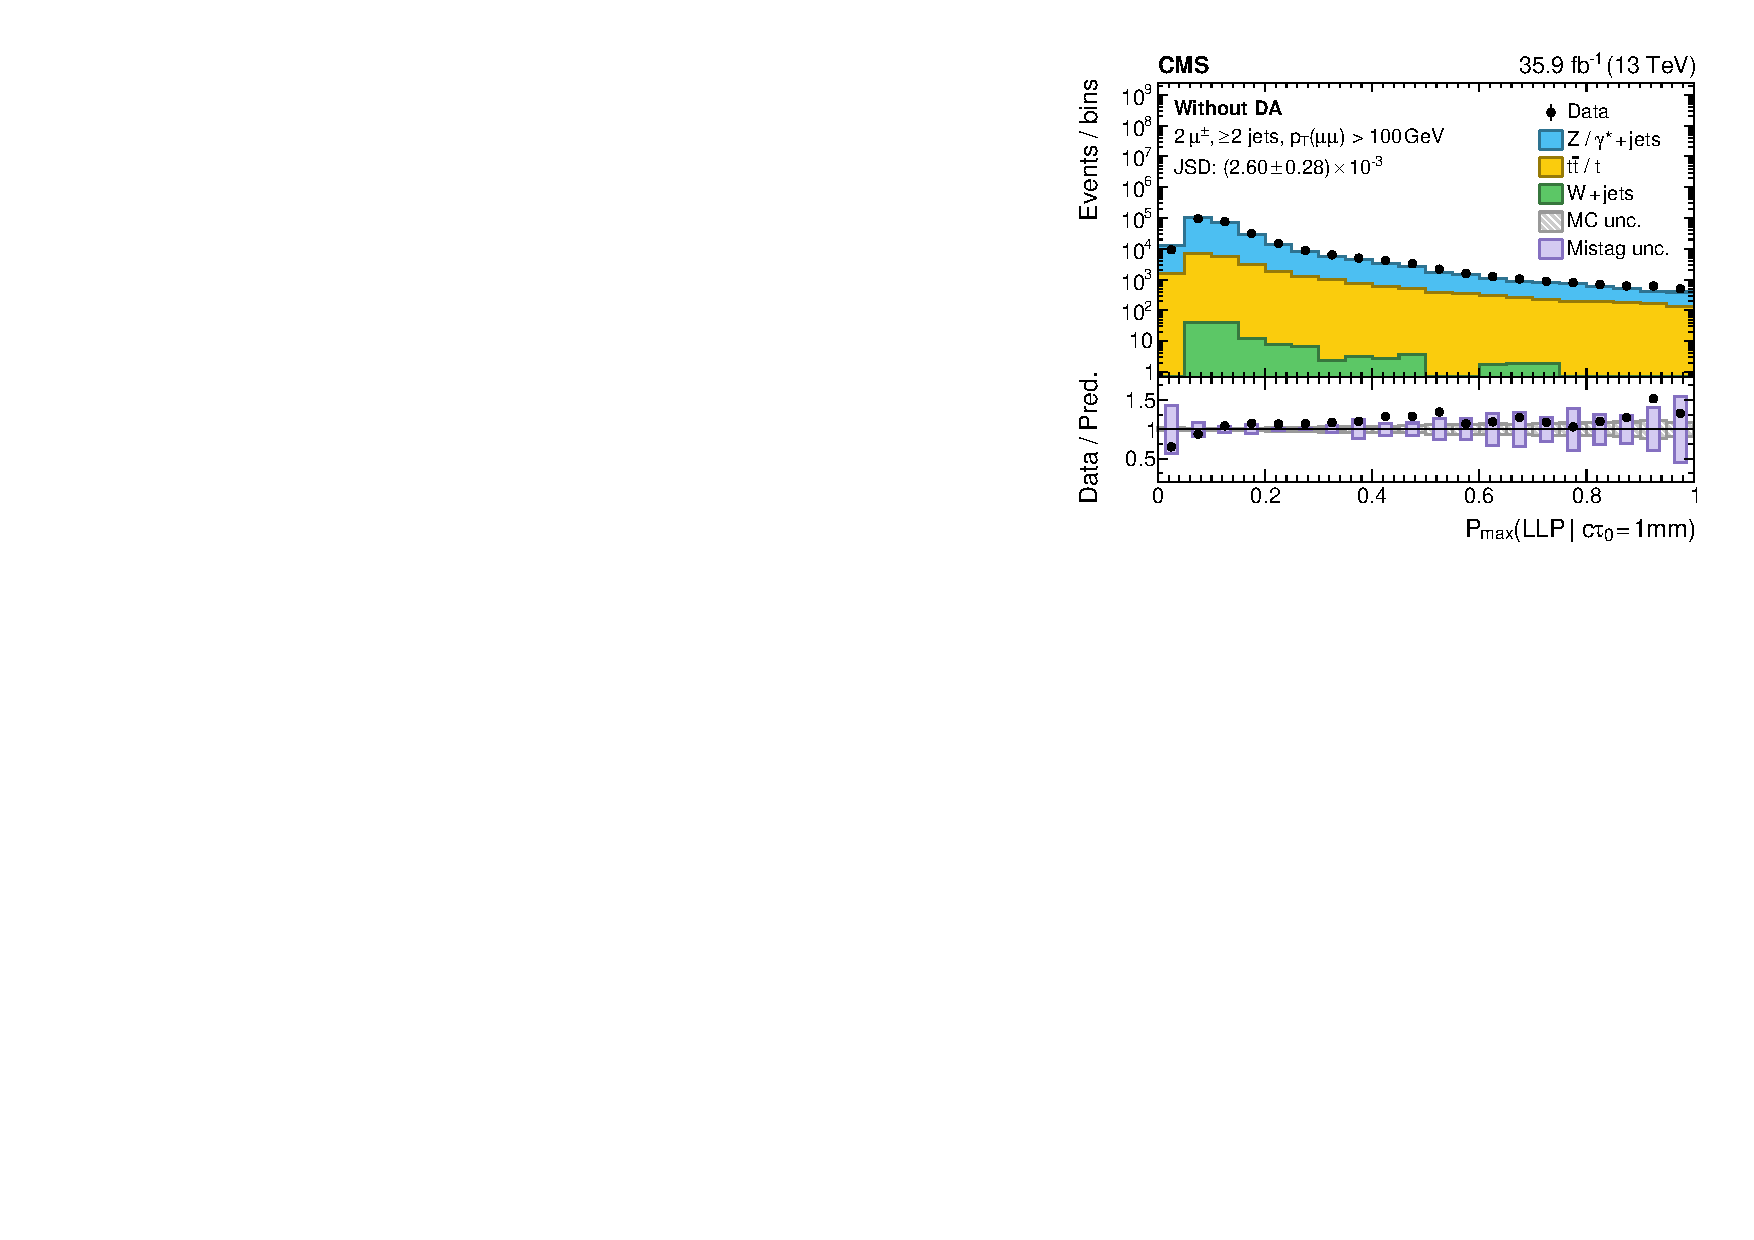
\includegraphics[width=0.48\textwidth]{figs/2mu_2toNj__llpdnnx_noda_0_max_highpt.pdf}\hspace{0.03\textwidth}
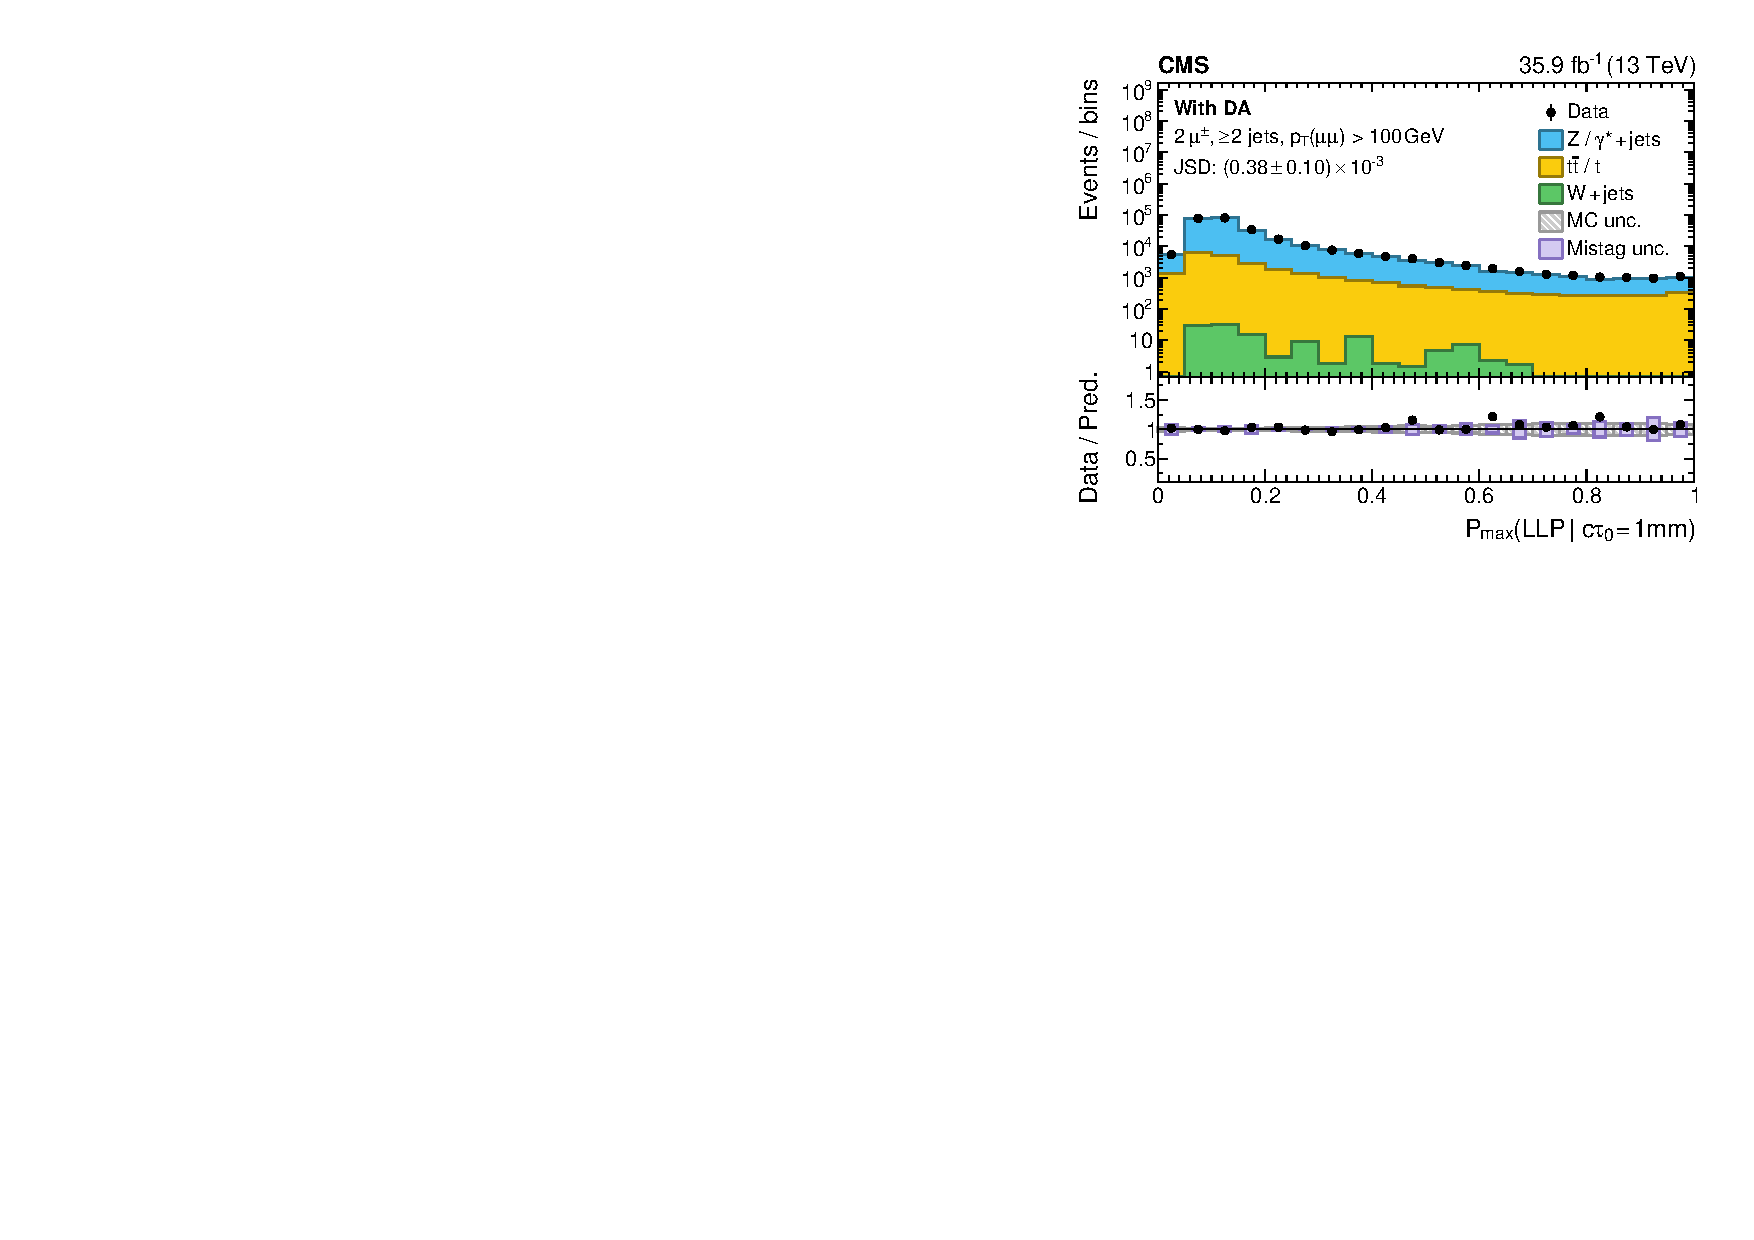
\includegraphics[width=0.48\textwidth]{figs/2mu_2toNj__llpdnnx_da_0_max_highpt.pdf}
\centering
\caption{The figures are taken from Ref.~\cite{CMS-EXO-19-011}.}
\label{fig-3}
\end{figure*}

\section{Performance}
\label{peformance}

\begin{figure*}[!ht]
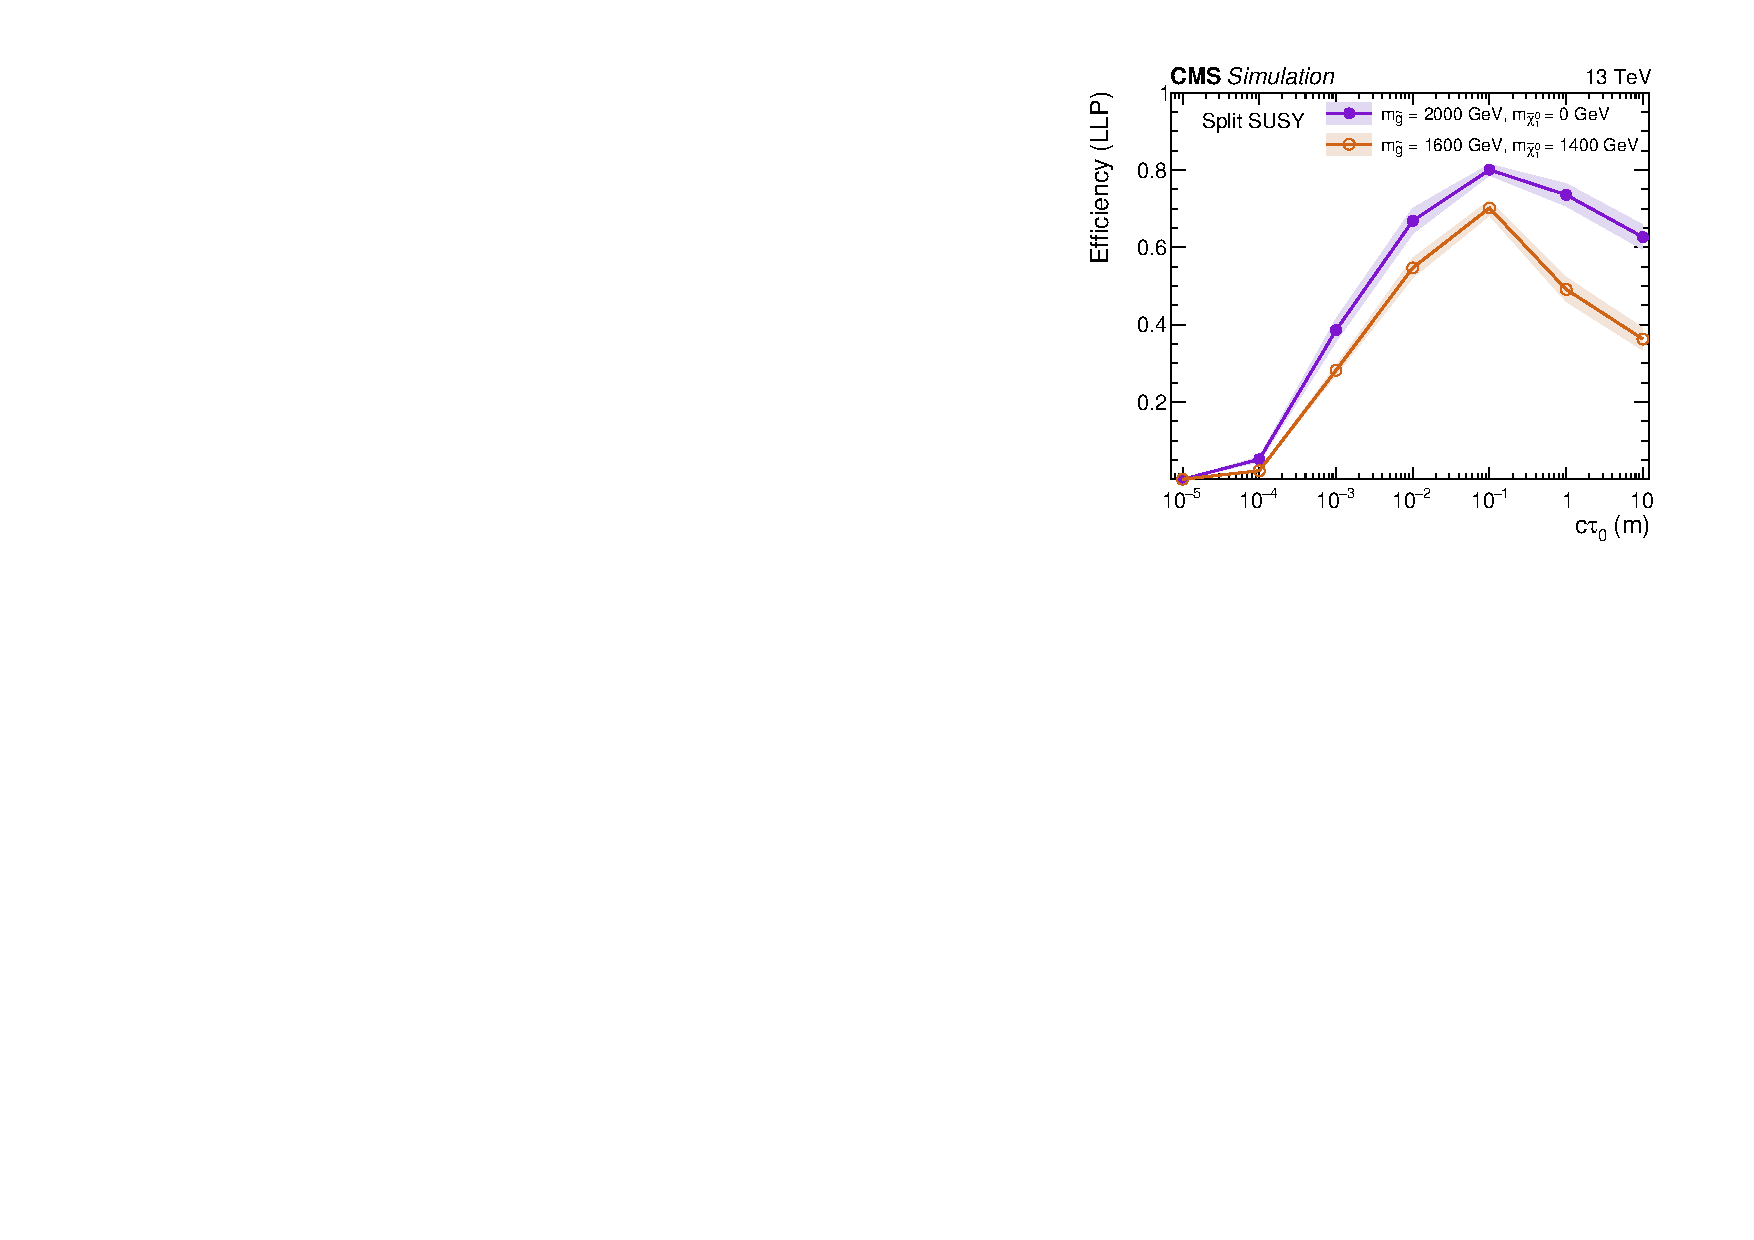
\includegraphics[width=0.48\textwidth]{figs/ctau.pdf}\hspace{0.03\textwidth}
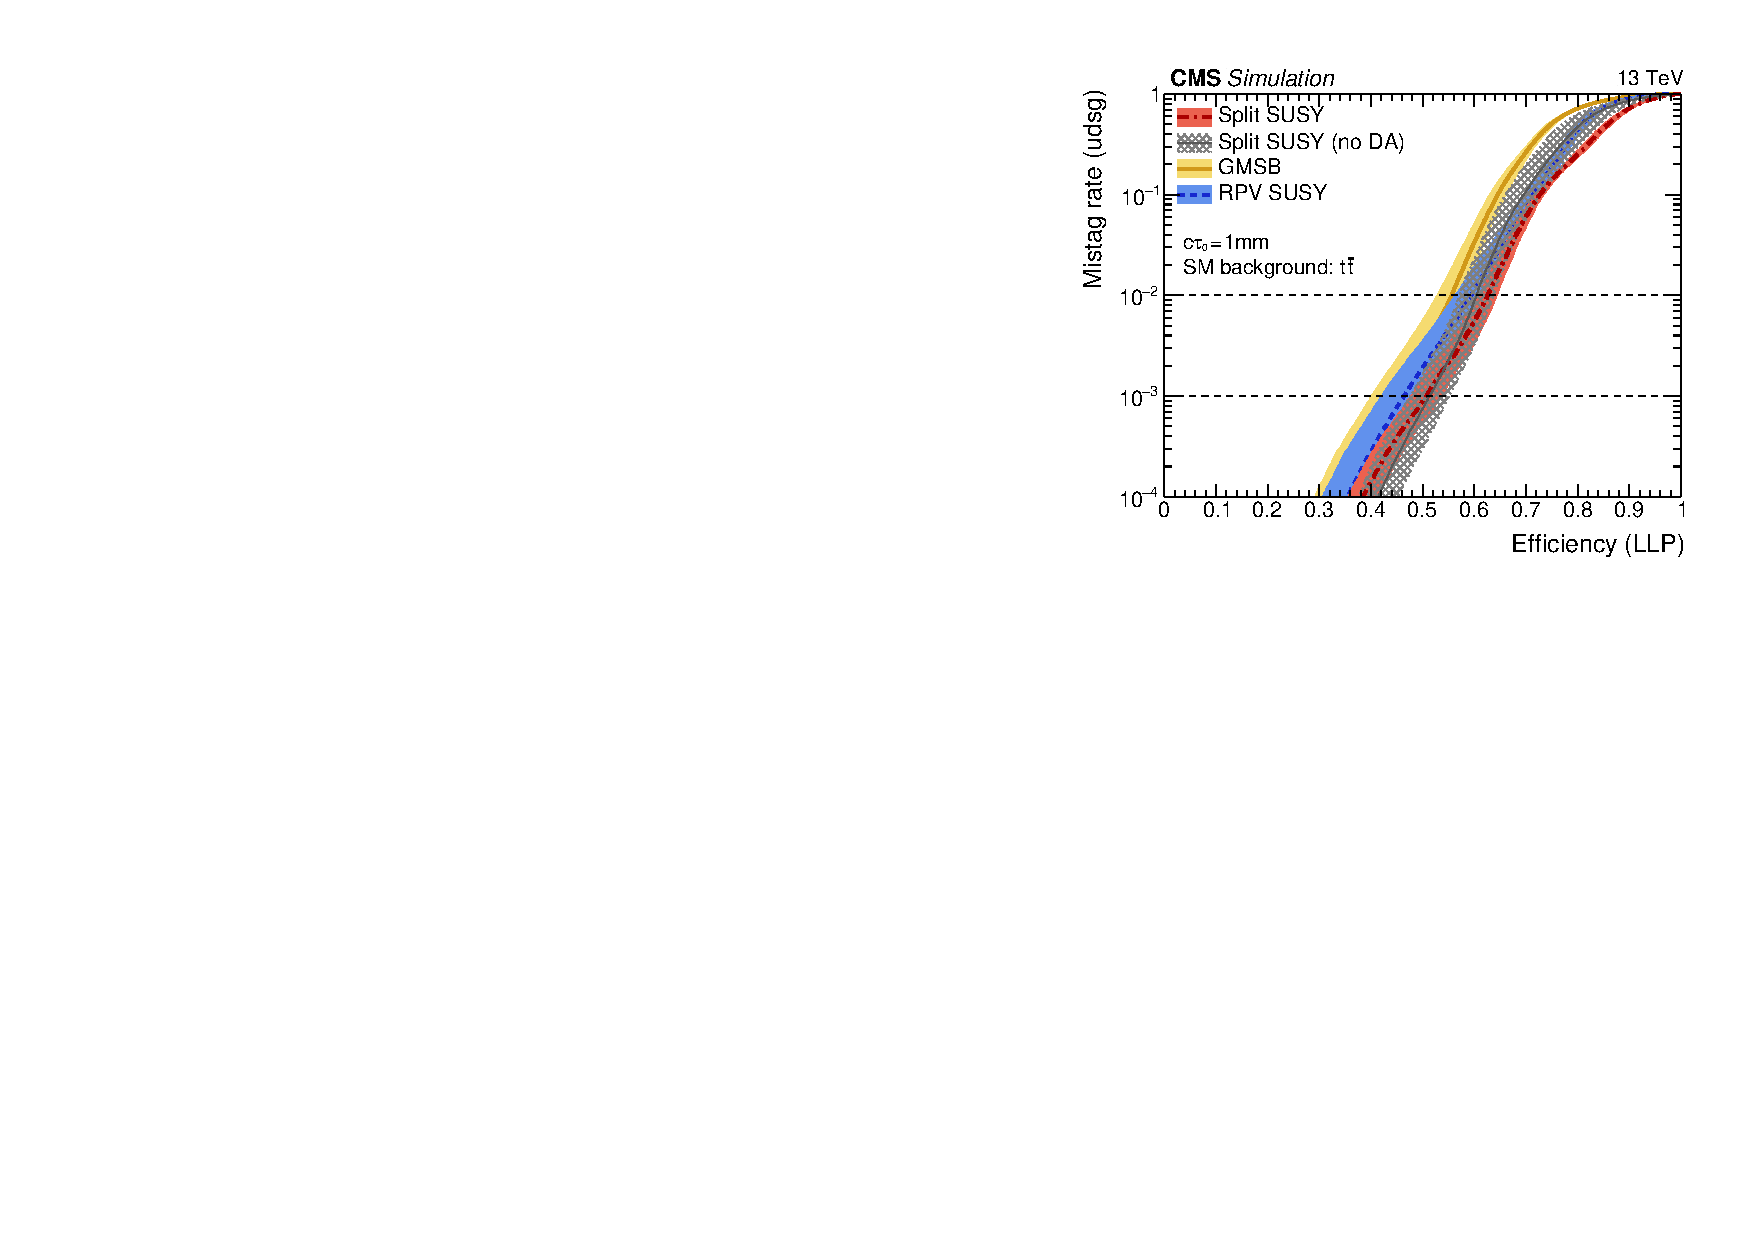
\includegraphics[width=0.48\textwidth]{figs/roc_1.pdf}
\centering
\caption{The figures are taken from Ref.~\cite{CMS-EXO-19-011}.}
\label{fig-3}
\end{figure*}

\section{Showcase search for long-lived gluinos}
\label{showcase}

\begin{figure*}[!ht]
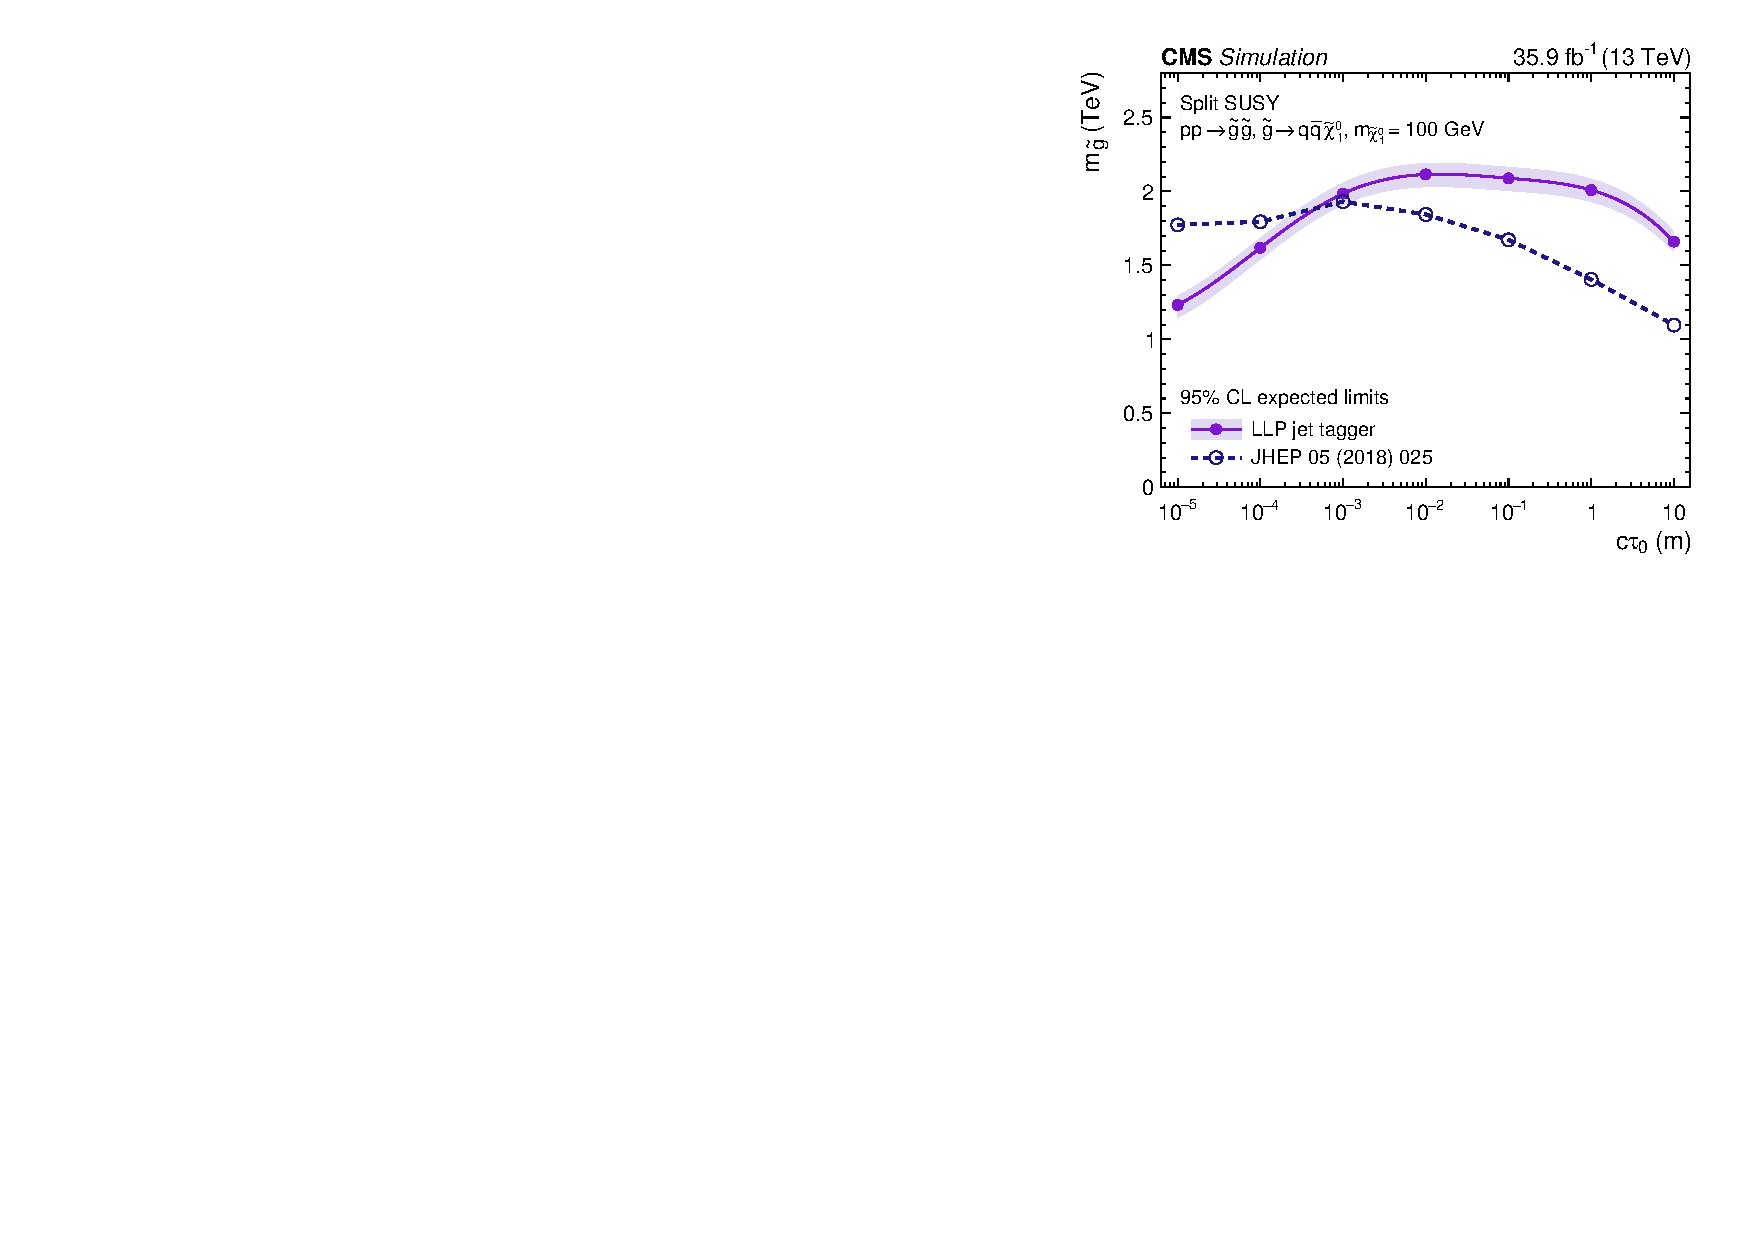
\includegraphics[width=0.48\textwidth]{figs/summaryU.pdf}\hspace{0.03\textwidth}
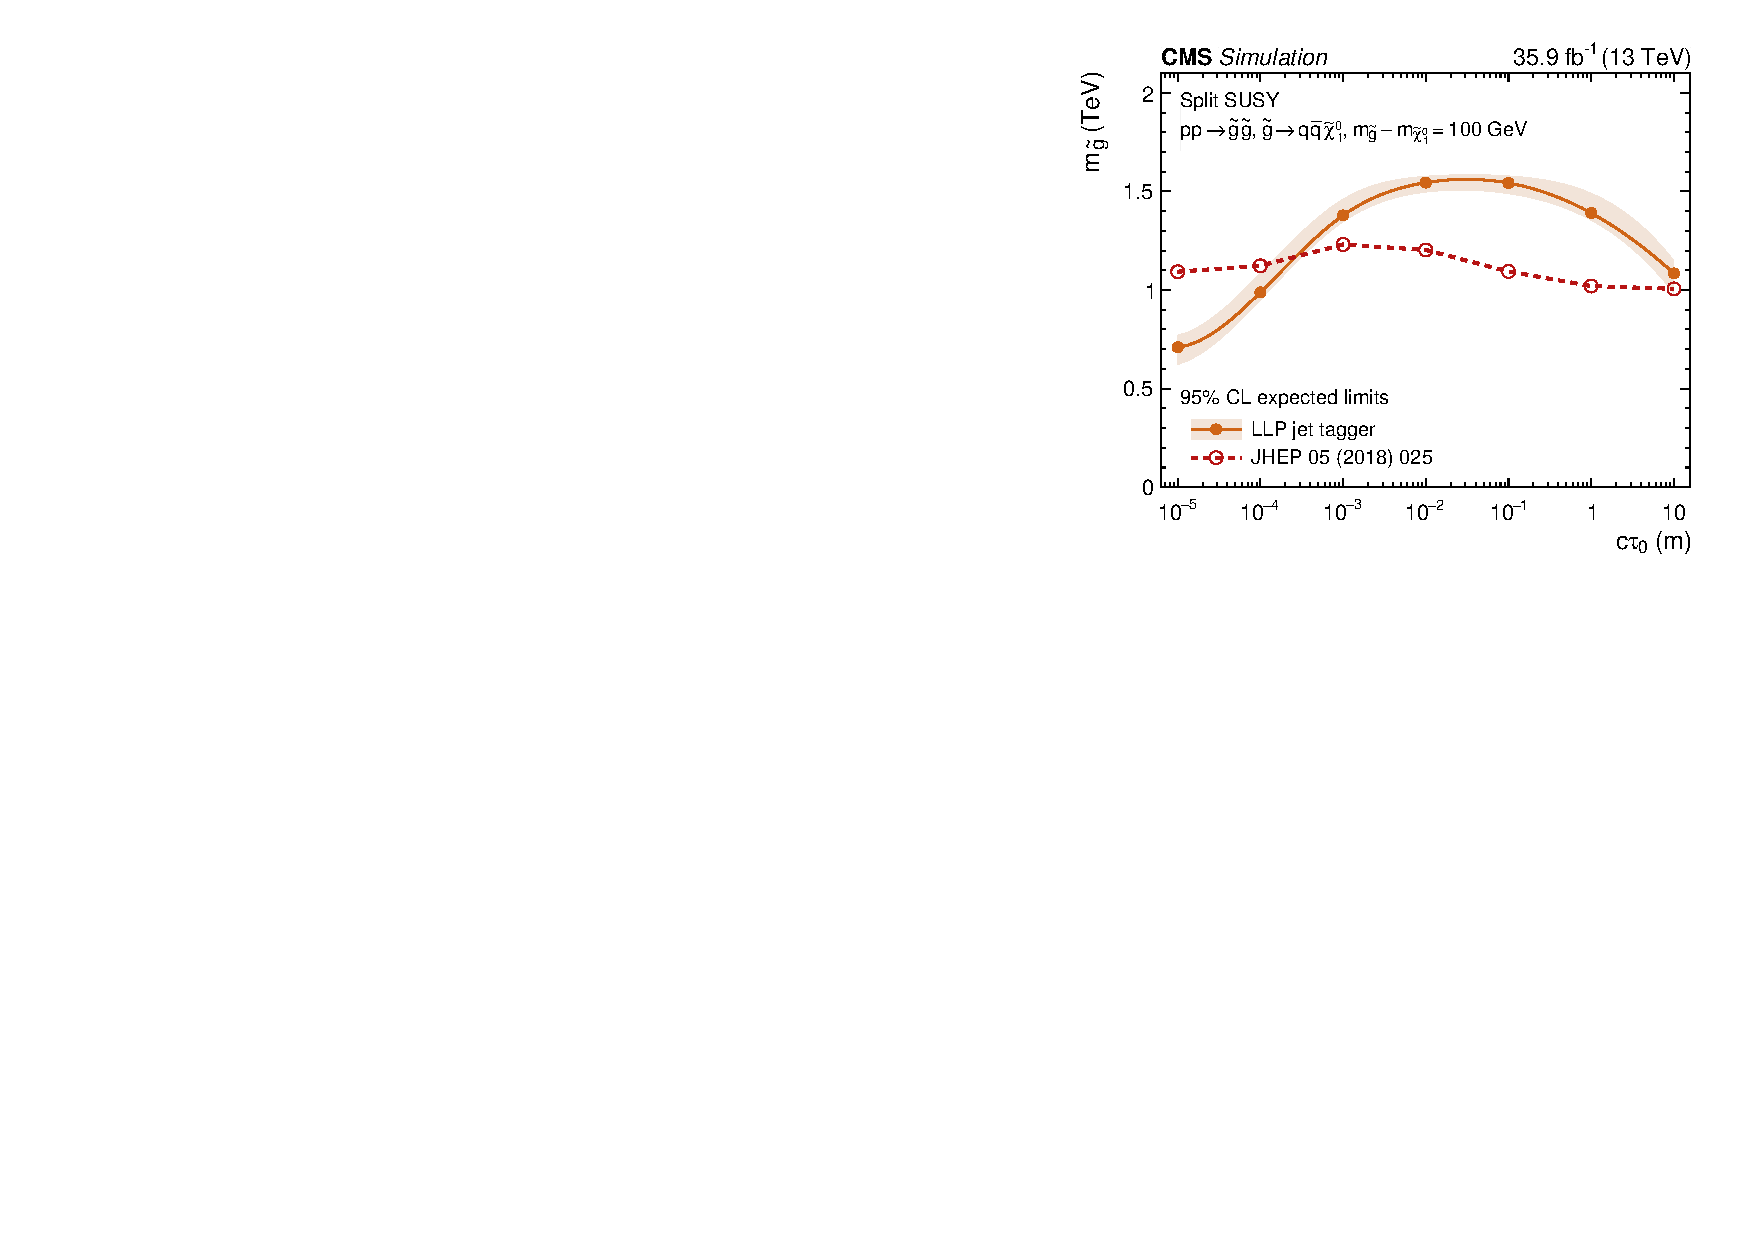
\includegraphics[width=0.48\textwidth]{figs/summaryC.pdf}
\centering
\caption{The figures are taken from Ref.~\cite{CMS-EXO-19-011}.}
\label{fig-4}
\end{figure*}

\section{Summary}
\label{Summary}


\clearpage

\begin{thebibliography}{}
\bibitem{ml-white-paper} K. Albertsson et al., J. Phys. Conf. Ser. \textbf{1085} (2018), 022008, \href{http://www.arxiv.org/abs/1807.02876}{arXiv:1807.02876}.

\bibitem{atlas} ATLAS Collaboration, JINST \textbf{3} (2008) S08003, \href{http://dx.doi.org/10.1088/1748-0221/3/08/S08003}{doi:10.1088/1748-0221/3/08/S08003}.

\bibitem{cms}  CMS Collaboration, JINST \textbf{3} (2008) S08004,
\href{http://dx.doi.org/10.1088/1748-0221/3/08/S08004}{doi:10.1088/1748-0221/3/08/S08004}.

\bibitem{batlas} ATLAS Collaboration, Eur. Phys. J. C \textbf{79} (2019) 970, \href{http://dx.doi.org/10.1140/epjc/s10052-019-7450-8}{doi:10.1140/epjc/s10052-019-7450-8}.

\bibitem{bcms} CMS Collaboration, JINST \textbf{13} (2018) P05011,
\href{http://dx.doi.org/10.1088/1748-0221/13/05/P05011}{doi:10.1088/1748-0221/13/05/P05011}.

\bibitem{CMS-EXO-19-011} CMS Collaboration, Submitted to MLST, (2019), \href{https://arxiv.org/abs/1912.12238}{arXiv:1912.12238}.

\bibitem{dj} CMS Collaboration, CMS-DP-2018-058, (2018), \href{https://cds.cern.ch/record/2646773}{cds.cern.ch/record/2646773}.

\bibitem{da} Y. Ganin et al., arXiv e-prints (2014), \href{https://arxiv.org/abs/1409.7495}{arXiv:1409.7495}.

\bibitem{splitsusy} J. L. Hewett et al., JHEP \textbf{09} (2004) 070, \href{http://dx.doi.org/10.1088/1126-6708/2004/09/070}{doi:10.1088/1126-6708/2004/09/070}.


\end{thebibliography}

\end{document}
